\documentclass{article}
\usepackage[utf8]{inputenc}
\usepackage[inline]{asymptote}
\usepackage{amsmath,amssymb,amsthm}

\usepackage{graphicx}

\title{2020 AMC 8 Problems and Solutions}
\author{Trung Nguyen}
\date{17 November 2020}

\begin{document}

\maketitle

\section{Problem 1}
Luka is making lemonade to sell at a school fundraiser. His recipe requires $4$ times as much water as sugar and twice as much sugar as lemon juice. He uses $3$ cups of lemon juice. How many cups of water does he need?

$\textbf{(A)}\ 6 \qquad \textbf{(B)}\ 8 \qquad \textbf{(C)}\ 12\qquad \textbf{(D)}\ 18 \qquad \textbf{(E)}\ 24$
\subsection{Solution}
We are given that $4w:s$ and $2s=l$ which we combine to get $8w:2s:l$. Letting all the variables equal $3$, we find that the answer is $3\cdot 8=\textbf{(E)}\ 24$.

\section{Problem 2}
Four friends do yardwork for their neighbors over the weekend, earning $\$15$, $\$20$, $\$25$, and $\$40$, respectively. They decide to split their earnings equally among themselves. In total how much will the friend who earned $\$40$ give to the others?

$\textbf{(A)}\ \$5 \qquad \textbf{(B)}\ \$10 \qquad \textbf{(C)}\ \$15\qquad \textbf{(D)}\ \$20 \qquad \textbf{(E)}\ \$25$
\subsection{Solution}
Notice that the friends have $\$15+\$20+\$25+\$40=\$100$ combined. Hence, they should each have $\frac{\$100}{4}=\$25$ if they are to slit the bounty equally. The answer then is $\$40-x=\$25 \Rightarrow x=\textbf{(C)}\ \$15 $. 

\section{Problem 3}
Carrie has a rectangular garden that measures $6$ feet by $8$ feet. She plants the entire garden with strawberry plants. Carrie is able to plant $4$ strawberry plants per square foot, and she harvests an average of $10$ strawberries per plant. How many strawberries can she expect to harvest?

$\textbf{(A)}\ 560 \qquad \textbf{(B)}\ 960 \qquad \textbf{(C)}\ 1120 \qquad \textbf{(D)}\ 1920 \qquad \textbf{(E)}\ 3840$
\subsection{Solution}
Note that $6\cdot 8 = 48$, so Carrie has $4\cdot 48 = 192$ strawberry plants. Each plant produces $10$ strawberries, so the final answer is $192\cdot 10 = \textbf{(D)}\ 1920$.

\section{Problem 4}
$4.$ Three hexagons of increasing size are shown below. Suppose the dot pattern continues so that each successive hexagon contains one more band of dots. How many dots are in the next hexagon?




\begin{figure}[ht]
\centering
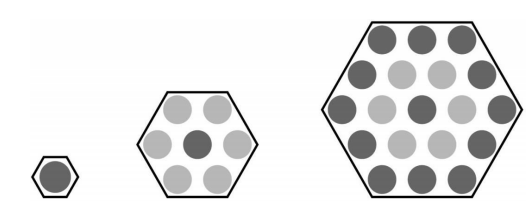
\includegraphics[width=.5\textwidth]{2020 AMC 8 Problem 4.png}

\end{figure}







$\textbf{(A) }35 \qquad \textbf{(B) }37 \qquad \textbf{(C) }39 \qquad \textbf{(D) }43 \qquad \textbf{(E) }49$
\subsection{Solution}
Let the hexagon with $1$ dot be $h_0$. Notice that the rest of the terms are generated by the recurrence relation $h_n=h_{n-1}+6n$ for $n> 0$. Using this, we find that $h_1=7,h_2=19,$ and $h_3=\textbf{(B) }37$.

\section{Problem 5}
Three fourths of a pitcher is filled with pineapple juice. The pitcher is emptied by pouring an equal amount of juice into each of $5$ cups. What percent of the total capacity of the pitcher did each cup receive?

$\textbf{(A) }5 \qquad \textbf{(B) }10 \qquad \textbf{(C) }15 \qquad \textbf{(D) }20 \qquad \textbf{(E) }25$
\subsection{Solution}
Notice that each cup receives $\frac 34 \cdot \frac 15=\frac{3}{20}=\frac{15}{100}$ of the entire pitcher which is $\textbf{(C) }15$ percent.

\section{Problem 6}
Aaron, Darren, Karen, Maren, and Sharon rode on a small train that has five cars that seat one person each. Maren sat in the last car. Aaron sat directly behind Sharon. Darren sat in one of the cars in front of Aaron. At least one person sat between Karen and Darren. Who sat in the middle car?

$\textbf{(A) }\text{Aaron} \qquad \textbf{(B) }\text{Darren} \qquad \textbf{(C) }\text{Karen} \qquad \textbf{(D) }\text{Maren}\qquad \textbf{(E) }\text{Sharon}$

\subsection{Solution}
Let the carts look like $$\_,\_,\_,\_,\_$$ where the left is the back and the right is the front. Using all the information given, it is not too hard to construct $$\text{M,K,A,S,D}$$ so the answer is $\textbf{(A) }\text{Aaron}$.
\section{Problem 7}
How many integers between $2020$ and $2400$ have four distinct digits arranged in increasing order? (For example, $2357$ is one such integer.)

$\textbf{(A) }9 \qquad \textbf{(B) }10 \qquad \textbf{(C) }15 \qquad \textbf{(D) }21 \qquad \textbf{(E) }28$
\subsection{Solution}
Notice that the number is of the form $23AB$ were $A>B>3$. We have $A=4,B\in [5,9];A=5,B\in [6,9];A=6,B\in [7,9];A=7,B\in [8,9];A=8,B\in [9]$. Counting the numbers in the brackets, the answer is $5+4+3+2+1=\textbf{(C) }15$.
\section{Problem 8}
Ricardo has $2020$ coins, some of which are pennies ($1$-cent coins) and the rest of which are nickels ($5$-cent coins). He has at least one penny and at least one nickel. What is the difference in cents between the greatest possible and least possible amounts of money that Ricardo can have?

$\textbf{(A) }8062 \qquad \textbf{(B) }8068 \qquad \textbf{(C) }8072 \qquad \textbf{(D) }8076 \qquad \textbf{(E) }8082$
\subsection{Solution}
The idea is maximizing the number of nickels and then maximizing the number of pennies, and then take their difference. This is given by $(2019\cdot 5+1)-(2019\cdot 1+5)=\textbf{(C) }8072$.
\section{Problem 9}
Akash's birthday cake is in the form of a $4 \times 4 \times 4$ inch cube. The cake has icing on the top and the four side faces, and no icing on the bottom. Suppose the cake is cut into $64$ smaller cubes, each measuring $1 \times 1 \times 1$ inch, as shown below. How many of the small pieces will have icing on exactly two sides?
\begin{figure}[ht]
\centering
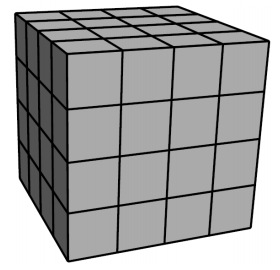
\includegraphics[width=.5\textwidth]{2020 AMC 8 Problem 9.png}

\end{figure}

$\textbf{(A) }12 \qquad \textbf{(B) }16 \qquad \textbf{(C) }18 \qquad \textbf{(D) }20 \qquad \textbf{(E) }24$
\subsection{Solution 9}
This is just careful casework. Consider the following diagram: 
\begin{figure}[ht]
\centering
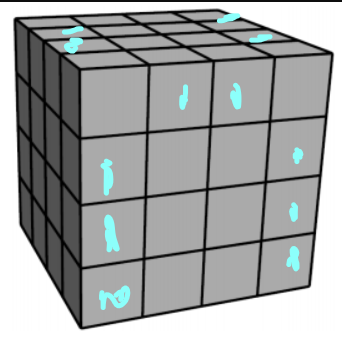
\includegraphics[width=.5\textwidth]{2020 AMC 8 Solution 9.png}

\end{figure}

The face on the opposite side of the front face (hidden) is an exact copy of the front face. So the answer is $8+4+8=\textbf{(D) }20$.
\section{Problem 10}
Zara has a collection of $4$ marbles: an Aggie, a Bumblebee, a Steelie, and a Tiger. She wants to display them in a row on a shelf, but does not want to put the Steelie and the Tiger next to one another. In how many ways can she do this?

$\textbf{(A) }6 \qquad \textbf{(B) }8 \qquad \textbf{(C) }12 \qquad \textbf{(D) }18 \qquad \textbf{(E) }24$
\subsection{Solution 1}
We use complementary counting: we will count the numbers of ways where Steelie and Tiger are together and subtract that from the total count. Treat the Steelie and the Tiger as a "super marble." There are $2!$ ways to arrange Steelie and Tiger within this "super marble." Then there are $3!$ ways to arrange the "super marble" and Zara's two other marbles in a row. Since there are $4!$ ways to arrange the marbles without any restrictions, the answer is given by $4!-2!\cdot 3!=\textbf{(C) }12$
\subsection{Solution 2}
We will use the following

\textbf{Georgeooga-Harryooga Theorem:} The Georgeooga-Harryooga Theorem states that if you have $a$ distinguishable objects and $b$ of them cannot be together, then there are $\frac{(a-b)!(a-b+1)!}{b!}$ ways to arrange the objects.

\textit{Proof. (translated by AoPS user RedFireTruck)}
Let our group of $a$ objects be represented like so $1$, $2$, $3$, ..., $a-1$, $a$. Let the last $b$ objects be the ones we can't have together.

Then we can organize our objects like so: $\_1\_2\_3\_...\_ a-b-1\_a-b\_$

We have $(a-b)!$ ways to arrange the objects in that list.

Now we have $a-b+1$ blanks so we have $_{a-b+1}P_{b}=\frac{(a-b+1)!}{(a-2b+1)!}$ ways to arrange the objects we can't put together

By fundamental counting principal our final answer is $\frac{(a-b)!(a-b+1)!}{(a-2b+1)!}$.$\square$

Back to the problem. By the Georgeooga-Harryooga Theorem, our answer is $\frac{(4-2)!(4-2+1)!}{(4-2\cdot2+1)!}=\textbf{(C) }12$.

\section{Problem 11}
After school, Maya and Naomi headed to the beach, $6$ miles away. Maya decided to bike while Naomi took a bus. The graph below shows their journeys, indicating the time and distance traveled. What was the difference, in miles per hour, between Naomi's and Maya's average speeds?

\begin{asy}
unitsize(1.25cm);
dotfactor = 10;
pen shortdashed=linetype(new real[] {2.7,2.7});

for (int i = 0; i < 6; ++i) {
for (int j = 0; j < 6; ++j) {
draw((i,0)--(i,6), grey);
draw((0,j)--(6,j), grey);
}
}

for (int i = 1; i <= 6; ++i) {
draw((-0.1,i)--(0.1,i),linewidth(1.25));
draw((i,-0.1)--(i,0.1),linewidth(1.25));
label(string(5*i), (i,0), 2*S);
label(string(i), (0, i), 2*W);
}

draw((0,0)--(0,6)--(6,6)--(6,0)--(0,0)--cycle,linewidth(1.25));

label(rotate(90) * "Distance (miles)", (-0.5,3), W);
label("Time (minutes)", (3,-0.5), S);

dot("Naomi", (2,6), 3*dir(305));
dot((6,6));

label("Maya", (4.45,3.5));

draw((0,0)--(1.15,1.3)--(1.55,1.3)--(3.15,3.2)--(3.65,3.2)--(5.2,5.2)--(5.4,5.2)--(6,6),linewidth(1.35));
draw((0,0)--(0.4,0.1)--(1.15,3.7)--(1.6,3.7)--(2,6),linewidth(1.35)+shortdashed);
\end{asy}


$\textbf{(A) }6 \qquad \textbf{(B) }12 \qquad \textbf{(C) }18 \qquad \textbf{(D) }20 \qquad \textbf{(E) }24$

\subsection{Solution}
Notice that Naomi travels at a rate of $6$ miles every $10$ minutes or $36$ miles an hour. Maya travels at a rate of $6$ miles every $30$ minutes or $12$ miles an hour. Hence, the answer is $36-12=\textbf{(E) }24$.
\section{Problem 12}
For positive integer $n$ , the factorial notation $n!$ represents the product of the integers from $n$ to $1$. (For example, $6! = 6 \cdot 5 \cdot 4 \cdot 3 \cdot 2 \cdot 1$.) What value of $N$ satisfies the following equation?$$5! \cdot 9! = 12 \cdot N!$$
$\textbf{(A)}10\qquad~~\textbf{(B)}11\qquad~~\textbf{(C)}12\qquad~~\textbf{(D)}13\qquad~~\textbf{(E)}14$
\subsection{Solution}
Notice that $5!\cdot 9!=12\cdot 10\cdot 9!=12\cdot 10!$. We are also told that $12\cdot 10!=12*N!$ from where it is obvious that $N=\textbf{(A)}10$.
\section{Problem 13}
Jamal has a drawer containing $6$ green socks, $18$ purple socks, and $12$ orange socks. After adding more purple socks, Jamal noticed that there is now a $60\%$ chance that a sock randomly selected from the drawer is purple. How many purple socks did Jamal add?

$\textbf{(A)}6\qquad~~\textbf{(B)}9\qquad~~\textbf{(C)}12\qquad~~\textbf{(D)}18\qquad~~\textbf{(E)}24$
\subsection{Solution}
Let Jamal add $x$ more purple socks. Then we are told that $\frac{18+x}{6+18+12+x}=\frac35$.  Cross multiplying and simplifying tells us that $x=\textbf{(B)}9$.
\section{Problem 14}
There are $20$ cities in the County of Newton. Their populations are shown in the bar chart below. The average population of all the cities is indicated by the horizontal dashed line. Which of the following is closest to the total population of all $20$ cities?


\begin{figure}[ht]
\centering
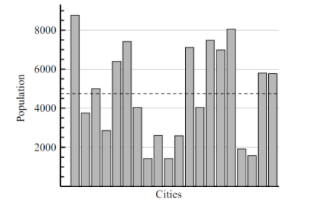
\includegraphics[width=.5\textwidth]{2020 AMC 8 Problem 14.png}
\end{figure}

$\textbf{(A) }65{,}000 \qquad \textbf{(B) }75{,}000 \qquad \textbf{(C) }85{,}000 \qquad \textbf{(D) }95{,}000 \qquad \textbf{(E) }105{,}000$
\subsection{Solution}
After reading the question, we notice that the dashed line is the average population of each city. Also, that dashed line is slightly less than $5\,000$. Since there are $20$ cities, the answer is slightly less than $20\cdot 5\,000\approx 100\,000$ which is closest to $\textbf{(D) }95{,}000$.
\section{Problem 15}
$15.$ Suppose $15\%$ of $x$ equals $20\%$ of $y.$ What percentage of $x$ is $y?$

$\textbf{(A) }5 \qquad \textbf{(B) }35 \qquad \textbf{(C) }75 \qquad \textbf{(D) }133 \frac13 \qquad \textbf{(E) }300$
\subsection{Solution}
We are given that $0.15x=0.20y$. Multiplying both sides by $100$ and dividing by $20$ tells us that $y = \frac 34x =0.75x=\textbf{(C) }75$.
\section{Problem 16}
Each of the points $A,B,C,D,E,$ and $F$ in the figure below represents a different digit from $1$ to $6.$ Each of the five lines shown passes through some of these points. The digits along each line are added to produce five sums, one for each line. The total of the five sums is $47.$ What is the digit represented by $B?$
\begin{figure}[ht]
\centering
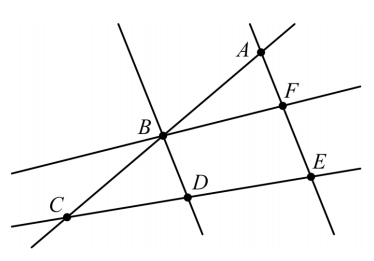
\includegraphics[width=.5\textwidth]{2020 AMC 8 Problem 16.png}
\end{figure}

$\textbf{(A) }1 \qquad \textbf{(B) }2 \qquad \textbf{(C) }3 \qquad \textbf{(D) }4 \qquad \textbf{(E) }5$
\subsection{Solution}
We can write an equation. We are given $2A+3B+2C+2D+2E+2F=47$ which simplifies to $2(A+B+C+D+E+F)+B=47$. Recall that each of $A,B,C,D,E,F$ are unique integers from $1$ to $6$. Hence, our equation simplifies to $42+B=47$ regardless of which letters equal which numbers. Now we can easily see that the answer is $\textbf{(E) }5$.
\section{Problem 17}
How many factors of 2020 have more than 3 factors? (As an example, 12 has 6 factors, namely 1, 2, 3, 4, 6, and 12.)

$\textbf{(A)}\ 6 \qquad \textbf{(B)}\ 7 \qquad \textbf{(C)}\ 8 \qquad \textbf{(D)}\ 9 \qquad \textbf{(E)}\ 10$
\subsection{Solution}
The prime factorization of $2020$ is $2^2\cdot5\cdot101$ so it has $(2+1)(1+1)(1+1)=12$ factors. Then we can count that $1,2,4,5,101$ all have $3$ or fewer divisors so by complementary counting our answer is $12-5=\textbf{(B)}\ 7$.
\section{Problem 18}
Rectangle $ABCD$ is inscribed in a semicircle with diameter $\overline{FE},$ as shown in the figure. Let $DA=16,$ and let $FD=AE=9.$ What is the area of $ABCD?$

\begin{figure}[ht]
\centering
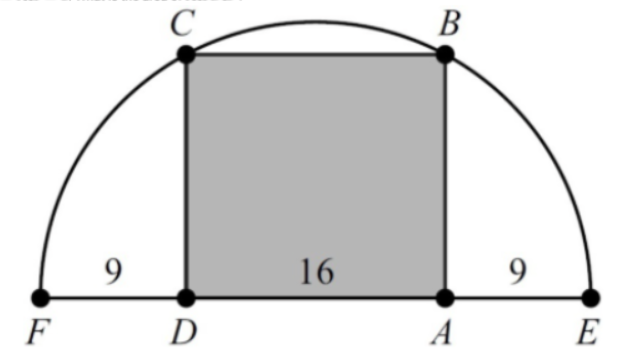
\includegraphics[width=.5\textwidth]{2020 AMC 8 Problem 18.png}
\end{figure}

$\textbf{(A) }240 \qquad \textbf{(B) }248 \qquad \textbf{(C) }256 \qquad \textbf{(D) }264 \qquad \textbf{(E) }272$
\subsection{Solution}
First, realize that $ABCD$ is not a square. Let $O$ be the midpoint of $FE$. Since $FE=9+9+16=34$, we have $OF=OE=\frac{34}{2}=17=OB$ because they are all radii. Since $O$ is also the midpoint of $AD$, we have $OA=\frac{16}2=8$. By the Pythagorean Theorem on $\triangle BAO$, we find that $AB=15$. The answer is then $16\cdot 15=\textbf{(A) }240$.
\section{Problem 19}
A number is called flippy if its digits alternate between two distinct digits. For example, $2020$ and $37373$ are flippy, but $3883$ and $123123$ are not. How many five-digit flippy numbers are divisible by $15?$

$\textbf{(A) }3 \qquad \textbf{(B) }4 \qquad \textbf{(C) }5 \qquad \textbf{(D) }6 \qquad \textbf{(E) }8$
\subsection{Solution}
A flippy number is of the form $5X5X5$ where $x\in\{0,3,6,9\}$ by the divisibility rules for $3$ and $5$ so the answer is $\textbf{(B) }4$.
\section{Problem 20}
A scientist walking through a forest recorded as integers the heights of $5$ trees standing in a row. She observed that each tree was either twice as tall or half as tall as the one to its right. Unfortunately some of her data was lost when rain fell on her notebook. Her notes are shown below, with blanks indicating the missing numbers. Based on her observations, the scientist was able to reconstruct the lost data. What was the average height of the trees, in meters?


    
\begin{tabular}{|c|c|}
\hline Tree 1 & \rule{0.2cm}{0.15mm} meters \\
Tree 2 & 11 meters \\
Tree 3 & \rule{0.2cm}{0.15mm} meters \\
Tree 4 & \rule{0.2cm}{0.15mm} meters \\
Tree 5 & \rule{0.2cm}{0.15mm} meters \\ \hline
Average height & \rule{0.2cm}{0.15mm}.2 meters \\
\hline
\end{tabular}


$\textbf{(A) }22.2 \qquad \textbf{(B) }24.2 \qquad \textbf{(C) }33.2 \qquad \textbf{(D) }35.2 \qquad \textbf{(E) }37.2$
\subsection{Solution}
The problem states that all tree heights are integers. Therefore, we can deduce that the first and third trees have a height of $22$ meters. Trees four and five must have heights of either $11,22$ or $44,88$ or $44,22$. Checking which ones match the answer choices, we find that the trees four and five have heights of $44$ and $22$ meters, respectively. Thus, the answer is $\frac{22+11+22+44+22}5=\textbf{(B) }24.2$.

\section{Problem 21}
A game board consists of $64$ squares that alternate in color between black and white. The figure below shows square $P$ in the bottom row and square $Q$ in the top row. A marker is placed at $P.$ A step consists of moving the marker onto one of the adjoining white squares in the row above. How many $7$-step paths are there from $P$ to $Q?$ (The figure shows a sample path.)

\begin{asy}
size(200);

int[] x = {6, 5, 4, 5, 6, 5, 6};
int[] y = {1, 2, 3, 4, 5, 6, 7};
int N = 7;

for (int i = 0; i < 8; ++i) {
for (int j = 0; j < 8; ++j) {
draw((i,j)--(i+1,j)--(i+1,j+1)--(i,j+1)--(i,j));
if ((i+j) % 2 == 0) {
filldraw((i,j)--(i+1,j)--(i+1,j+1)--(i,j+1)--(i,j)--cycle,black);
}
}
}

for (int i = 0; i < N; ++i) {
draw(circle((x[i],y[i])+(0.5,0.5),0.35));
}

label("$P$", (5.5, 0.5));
label("$Q$", (6.5, 7.5));
\end{asy}

$\textbf{(A) }28 \qquad \textbf{(B) }30 \qquad \textbf{(C) }32 \qquad \textbf{(D) }33 \qquad \textbf{(E) }35$
\subsection{Solution}
The easiest way to solve this problem is just writing out the steps to get to each square as follows:

\begin{asy}
size(200);
int N = 7;
for (int i = 0; i < 8; ++i) {
for (int j = 0; j < 8; ++j) {
draw((i,j)--(i+1,j)--(i+1,j+1)--(i,j+1)--(i,j));
if ((i+j) % 2 == 0) {
filldraw((i,j)--(i+1,j)--(i+1,j+1)--(i,j+1)--(i,j)--cycle,black);
}
}
}
label("$1$", (5.5, .5));
label("$1$", (4.5, 1.5));
label("$1$", (6.5, 1.5));
label("$1$", (3.5, 2.5));
label("$1$", (7.5, 2.5));
label("$2$", (5.5, 2.5));
label("$1$", (2.5, 3.5));
label("$3$", (6.5, 3.5));
label("$3$", (4.5, 3.5));
label("$4$", (3.5, 4.5));
label("$3$", (7.5, 4.5));
label("$6$", (5.5, 4.5));
label("$10$", (4.5, 5.5));
label("$9$", (6.5, 5.5));
label("$19$", (5.5, 6.5));
label("$9$", (7.5, 6.5));
label("$28$", (6.5, 7.5));
\end{asy}

The answer is thus $\textbf{(A) }28$. Interestingly, the final answer is also $\binom 82...$
\section{Problem 22}
When a positive integer $N$ is fed into a machine, the output is a number calculated according to the rule shown below.

\begin{asy}
size(200);
defaultpen(linewidth(0.8)+fontsize(13));
real r = 0.05;
draw((0.9,0)--(3.5,0),EndArrow(size=7));
filldraw((4,2.5)--(7,2.5)--(7,-2.5)--(4,-2.5)--cycle,gray(0.65));
fill(circle((5.5,1.25),0.8),white);
fill(circle((5.5,1.25),0.5),gray(0.65));
fill((4.3,-r)--(6.7,-r)--(6.7,-1-r)--(4.3,-1-r)--cycle,white);
fill((4.3,-1.25+r)--(6.7,-1.25+r)--(6.7,-2.25+r)--(4.3,-2.25+r)--cycle,white);
fill((4.6,-0.25-r)--(6.4,-0.25-r)--(6.4,-0.75-r)--(4.6,-0.75-r)--cycle,gray(0.65));
fill((4.6,-1.5+r)--(6.4,-1.5+r)--(6.4,-2+r)--(4.6,-2+r)--cycle,gray(0.65));
label("$N$",(0.45,0));
draw((7.5,1.25)--(11.25,1.25),EndArrow(size=7));
draw((7.5,-1.25)--(11.25,-1.25),EndArrow(size=7));
label("if $N$ is even",(9.25,1.25),N);
label("if $N$ is odd",(9.25,-1.25),N);
label("$\displaystyle\frac N2$",(12,1.25));
label("$3N+1$",(12.6,-1.25));
\end{asy}

For example, starting with an input of $N=7,$ the machine will output $3 \cdot 7 +1 = 22.$ Then if the output is repeatedly inserted into the machine five more times, the final output is $26.$
$$7 \to 22 \to 11 \to 34 \to 17 \to 52 \to 26$$When the same $6$-step process is applied to a different starting value of $N,$ the final output is $1.$ What is the sum of all such integers $N?$
$$N \to \rule{0.5cm}{0.15mm} \to \rule{0.5cm}{0.15mm} \to \rule{0.5cm}{0.15mm} \to \rule{0.5cm}{0.15mm} \to \rule{0.5cm}{0.15mm} \to 1$$
$\textbf{(A) }73 \qquad \textbf{(B) }74 \qquad \textbf{(C) }75 \qquad \textbf{(D) }82 \qquad \textbf{(E) }83$
\subsection{Solution}
The most straightforward solutions is just working backwards with a diagram as shown below:

\begin{figure}[ht]
\centering
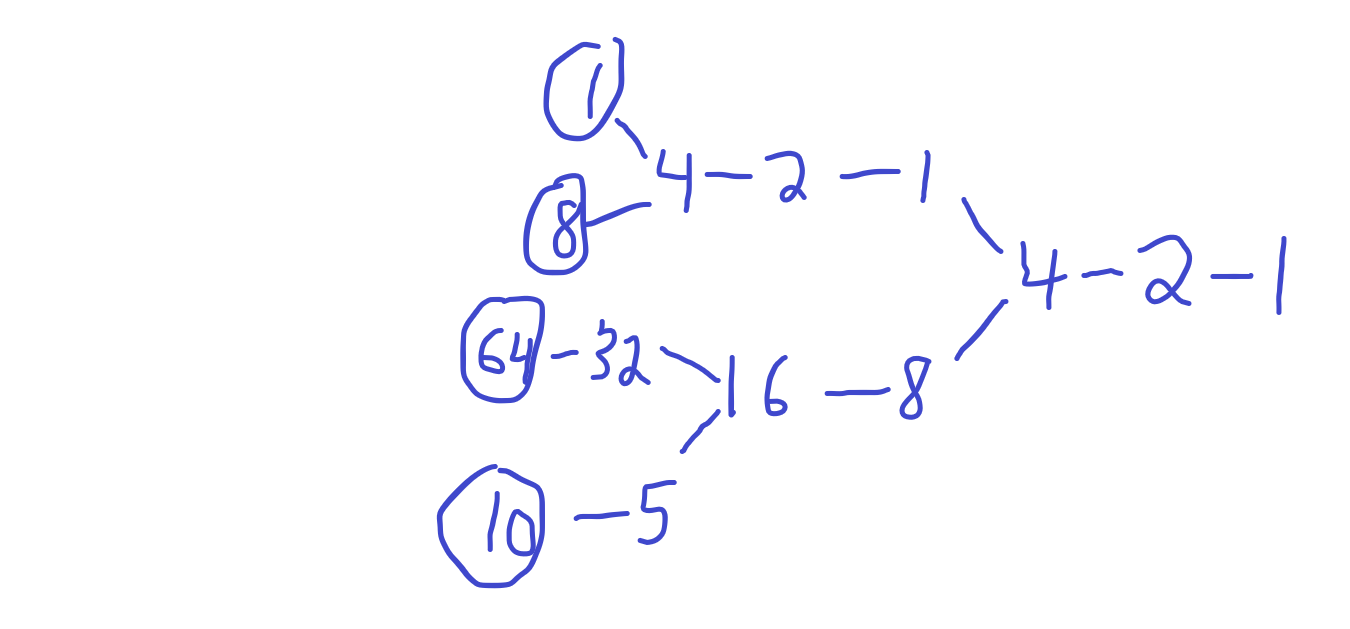
\includegraphics[width=.5\textwidth]{2020 AMC 8 Solution 22.png}

\end{figure}

Hence, the answer is $1+8+64+10=\textbf{(E) }83$.


\section{Problem 23}
$23.$ Five different awards are to be given to three students. Each student will receive at least one
award. In how many different ways can the awards be distributed?

$\textbf{(A) }120 \qquad \textbf{(B) }150 \qquad \textbf{(C) }180 \qquad \textbf{(D) }210 \qquad \textbf{(E) }240$
\subsection{Solution}
We can distribute the awards in a $3-1-1$ or $1-2-2$. We will handle each case separately.
For the first case, there are $\binom53 \cdot \binom21 \cdot \binom11 \cdot \frac{3!}{2!} = 60$ ways to distribute the prizes.

For the second case, there are $\binom52 \cdot \binom32 \cdot \binom11 \cdot \frac{3!}{2!}  = 90$ ways to distribute the prizes.

Therefore, the answer is $60 + 90 = \textbf{(B) }150$.

\section{Problem 24}
A large square region is paved with $n^2$ gray square tiles, each measuring $s$ inches on a side. A border $d$ inches wide surrounds each tile. The figure below shows the case for $n = 3$. When $n = 24$, the $576$ gray tiles cover $64\%$ of the area of the large square region. What is the ratio $\frac{d}{s}$ for this larger value of $n$?
\begin{asy}
size(100);
draw((0,0)--(13,0)--(13,13)--(0,13)--cycle);
filldraw((1,1)--(4,1)--(4,4)--(1,4)--cycle, mediumgray);
filldraw((1,5)--(4,5)--(4,8)--(1,8)--cycle, mediumgray);
filldraw((1,9)--(4,9)--(4,12)--(1,12)--cycle, mediumgray);
filldraw((5,1)--(8,1)--(8,4)--(5,4)--cycle, mediumgray);
filldraw((5,5)--(8,5)--(8,8)--(5,8)--cycle, mediumgray);
filldraw((5,9)--(8,9)--(8,12)--(5,12)--cycle, mediumgray);
filldraw((9,1)--(12,1)--(12,4)--(9,4)--cycle, mediumgray);
filldraw((9,5)--(12,5)--(12,8)--(9,8)--cycle, mediumgray);
filldraw((9,9)--(12,9)--(12,12)--(9,12)--cycle, mediumgray);
\end{asy}

$\textbf{(A)} \frac{6}{25} \qquad~~\textbf{(B)} \frac14 \qquad~~\textbf{(C)} \frac{9}{25} \qquad~~\textbf{(D)}\frac{7}{16} \qquad~~\textbf{(E)}\frac{9}{16}$
\subsection{Solution}
The area of the shaded region is $(24s)^2$. The total area of the square is $(24s+25d)^2$ because for each side of the square there one extra row/column of the boarder. Our equation is $\frac{(24s)^2}{(24x+25d)^2}=\frac{64}{100}$. Taking the square root of both sides gives $\frac{24x}{24x+25d}=\frac 45$. Cross multiplying and rearranging gives $\frac ds=\textbf{(A)} \frac{6}{25}$.
\section{Problem 25}
 Rectangles $R_1$ and $R_2,$ and squares $S_1,\,S_2,\,$ and $S_3,$ shown below, combine to form a rectangle that is 3322 units wide and 2020 units high. What is the side length of $S_2$ in units?

\begin{asy}
size(100);
draw((0,0)--(5,0)--(5,3)--(0,3)--(0,0));
draw((3,0)--(3,1)--(0,1));
draw((3,1)--(3,2)--(5,2));
draw((3,2)--(2,2)--(2,1)--(2,3));
label("$R_1$",(3/2,1/2));
label("$S_3$",(4,1));
label("$S_2$",(5/2,3/2));
label("$S_1$",(1,2));
label("$R_2$",(7/2,5/2));
\end{asy}

$\textbf{(A) }651 \qquad \textbf{(B) }655 \qquad \textbf{(C) }656 \qquad \textbf{(D) }662 \qquad \textbf{(E) }666$
\subsection{Solution}

WLOG, assume that $S_1=S_3$ and $R_1=R_2$. Let the sum of the lengths of $S_1$ and $S_3$ be $x$ and let the length of $S_2$ be $y$. We have the system \begin{align*}
    x+y&=3322\\
    x-y&=2020
\end{align*}
which we solve to find that $y=\textbf{(A) }651$.



\begin{figure}[ht]
\centering

\includegraphics[width=.5\textwidth]{maa logo.png}
\end{figure}

These problems are copyright $\copyright$ Mathematical Association of America
(www.maa.org)


\end{document}
